\RequirePackage{xcolor}
\documentclass[a0,24pt]{sciposter}
\usepackage[utf8]{inputenc}
\usepackage{lipsum}
\usepackage{tikz}
\usetikzlibrary{arrows.meta}
\usepackage{pgfplots}
\usepackage{pgfplotstable}
\usepackage[hidelinks]{hyperref}
\pgfplotsset{compat=newest} 
\usepgfplotslibrary{units} 
\usepackage{float}
\usepackage{multicol}
\usepackage{mathtools}
\usepackage{amsmath}
\usepackage{amsfonts}
\usepackage{caption}

%We need 24pt font. I also think we should cut the three sections down to two instead and make it make it stretch across the whole page. It will be a paper of size A0. Probably larger line spacing and larger font in the section headers. Move the title to the top of the left section and but information about us in the bottom right along with an SDU logo from here: http://www.sdu.dk/aktuelt/presserummet/logo_og_designguide/download. As well as our project name/number. 
\leftlogo{sdu-logo.png}
\title{Reaching Time Consensus with ATS and MMTS}
\date{\today}
\author{Johan Ringmann Fagerberg, Marcus Møller, Lucas Olai Jarlkov Olsen,\\
  Peter Heilbo Ratgen, Thomas Stenhaug}
\institute{Institut for Matematik og Datalogi\\
            Syddansk Universitet}
\email{moell17@student.sdu.dk, tsten16@student.sdu.dk, OTHER EMAILS}

\begin{document}

\maketitle

\begin{multicols}{2}

%Don't think we want an abstract here.

\section{Introduction}

Having a network of nodes agree on the current time isn't a trivial task. A proper solution has to not only achieve synchronization throughout the network, but has to do so despite communication delay in the network, nodes disappearing or reappearing, or potentially malicious nodes that attempt to throw off the synchronization.

The common method of time synchronization is having one or more nodes decide on the current ``true'' time, and propagating this throughout the network. This is an example of a non-consensus algorithm, which are particularly fragile to nodes going offline or being malicious.

A recently popularized alternative is consensus-based algorithms, in which no nodes are more important than any others. In these algorithms a consensus must be reached amongst the nodes, until the entire network eventually agrees on a shared time value. As all nodes carry the same weights, these algorithms are highly resistant to topology changes and malicious nodes.

%Graphs to illustrate the difference between a fully distributed system and a tree structure network.
\begin{figure}[h!]
    \centering
    \captionsetup{type=figure,width=0.7\textwidth,justification=centering}
    % Generated by https://goo.gl/RRAu5U
    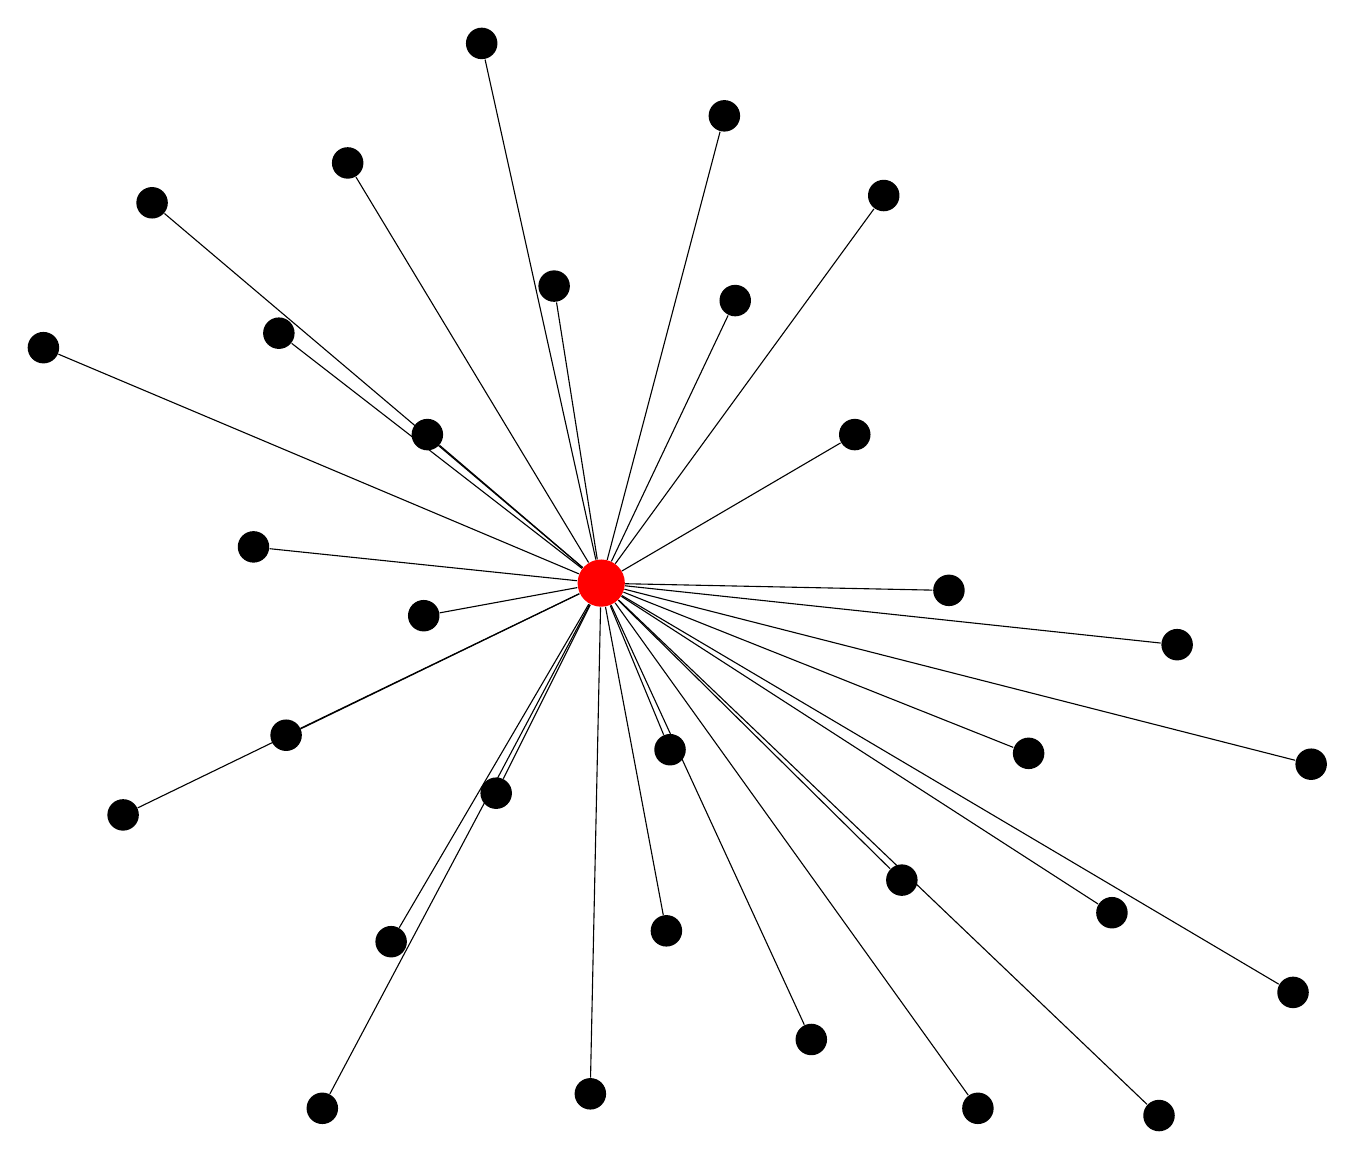
\begin{tikzpicture}[inner sep=0pt,minimum size=0.4cm,scale=4.6]
        \draw (2.00, 1.50) node[fill,circle,red,minimum size=0.6cm](master) {};
\draw (2.19, 1.04) node[fill,circle](node1) {};
\draw (master) -- (node1);
\draw (2.18, 0.54) node[fill,circle](node2) {};
\draw (master) -- (node2);
\draw (2.58, 0.24) node[fill,circle](node3) {};
\draw (master) -- (node3);
\draw (3.04, 0.05) node[fill,circle](node4) {};
\draw (master) -- (node4);
\draw (3.54, 0.03) node[fill,circle](node5) {};
\draw (master) -- (node5);
\draw (1.71, 0.92) node[fill,circle](node6) {};
\draw (master) -- (node6);
\draw (2.83, 0.68) node[fill,circle](node7) {};
\draw (master) -- (node7);
\draw (1.51, 1.41) node[fill,circle](node8) {};
\draw (master) -- (node8);
\draw (3.18, 1.03) node[fill,circle](node9) {};
\draw (master) -- (node9);
\draw (3.59, 1.33) node[fill,circle](node10) {};
\draw (master) -- (node10);
\draw (2.96, 1.48) node[fill,circle](node11) {};
\draw (master) -- (node11);
\draw (1.52, 1.91) node[fill,circle](node12) {};
\draw (master) -- (node12);
\draw (1.11, 2.19) node[fill,circle](node13) {};
\draw (master) -- (node13);
\draw (0.76, 2.55) node[fill,circle](node14) {};
\draw (master) -- (node14);
\draw (3.41, 0.59) node[fill,circle](node15) {};
\draw (master) -- (node15);
\draw (1.13, 1.08) node[fill,circle](node16) {};
\draw (master) -- (node16);
\draw (1.30, 2.66) node[fill,circle](node17) {};
\draw (master) -- (node17);
\draw (3.96, 1.00) node[fill,circle](node18) {};
\draw (master) -- (node18);
\draw (1.97, 0.09) node[fill,circle](node19) {};
\draw (master) -- (node19);
\draw (2.70, 1.91) node[fill,circle](node20) {};
\draw (master) -- (node20);
\draw (1.04, 1.60) node[fill,circle](node21) {};
\draw (master) -- (node21);
\draw (0.46, 2.15) node[fill,circle](node22) {};
\draw (master) -- (node22);
\draw (2.37, 2.28) node[fill,circle](node23) {};
\draw (master) -- (node23);
\draw (1.87, 2.32) node[fill,circle](node24) {};
\draw (master) -- (node24);
\draw (2.78, 2.57) node[fill,circle](node25) {};
\draw (master) -- (node25);
\draw (1.42, 0.51) node[fill,circle](node26) {};
\draw (master) -- (node26);
\draw (1.23, 0.05) node[fill,circle](node27) {};
\draw (master) -- (node27);
\draw (2.34, 2.79) node[fill,circle](node28) {};
\draw (master) -- (node28);
\draw (0.68, 0.86) node[fill,circle](node29) {};
\draw (master) -- (node29);
\draw (1.67, 2.99) node[fill,circle](node30) {};
\draw (master) -- (node30);
\draw (3.91, 0.37) node[fill,circle](node31) {};
\draw (master) -- (node31);
    \end{tikzpicture}
    \hspace{2em}
    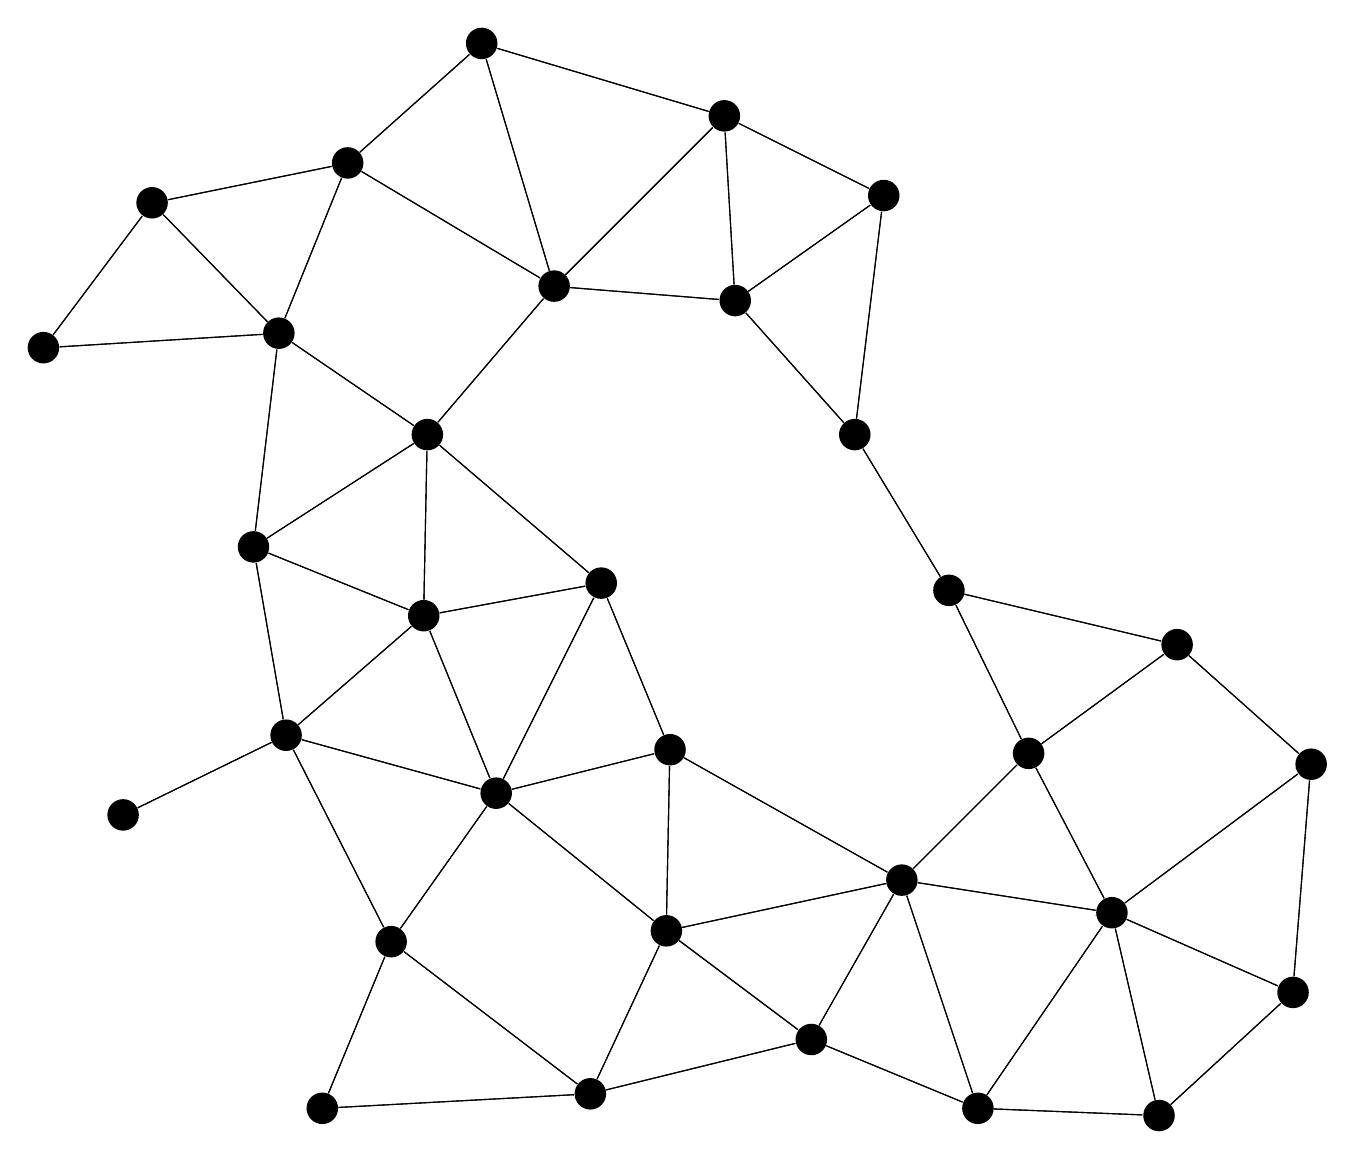
\begin{tikzpicture}[inner sep=0pt,minimum size=0.4cm,scale=4.6]
        \draw (2.00, 1.50) node[fill,circle](node0) {};
\draw (2.19, 1.04) node[fill,circle](node1) {};
\draw (2.18, 0.54) node[fill,circle](node2) {};
\draw (2.58, 0.24) node[fill,circle](node3) {};
\draw (3.04, 0.05) node[fill,circle](node4) {};
\draw (3.54, 0.03) node[fill,circle](node5) {};
\draw (1.71, 0.92) node[fill,circle](node6) {};
\draw (2.83, 0.68) node[fill,circle](node7) {};
\draw (1.51, 1.41) node[fill,circle](node8) {};
\draw (3.18, 1.03) node[fill,circle](node9) {};
\draw (3.59, 1.33) node[fill,circle](node10) {};
\draw (2.96, 1.48) node[fill,circle](node11) {};
\draw (1.52, 1.91) node[fill,circle](node12) {};
\draw (1.11, 2.19) node[fill,circle](node13) {};
\draw (0.76, 2.55) node[fill,circle](node14) {};
\draw (3.41, 0.59) node[fill,circle](node15) {};
\draw (1.13, 1.08) node[fill,circle](node16) {};
\draw (1.30, 2.66) node[fill,circle](node17) {};
\draw (3.96, 1.00) node[fill,circle](node18) {};
\draw (1.97, 0.09) node[fill,circle](node19) {};
\draw (2.70, 1.91) node[fill,circle](node20) {};
\draw (1.04, 1.60) node[fill,circle](node21) {};
\draw (0.46, 2.15) node[fill,circle](node22) {};
\draw (2.37, 2.28) node[fill,circle](node23) {};
\draw (1.87, 2.32) node[fill,circle](node24) {};
\draw (2.78, 2.57) node[fill,circle](node25) {};
\draw (1.42, 0.51) node[fill,circle](node26) {};
\draw (1.23, 0.05) node[fill,circle](node27) {};
\draw (2.34, 2.79) node[fill,circle](node28) {};
\draw (0.68, 0.86) node[fill,circle](node29) {};
\draw (1.67, 2.99) node[fill,circle](node30) {};
\draw (3.91, 0.37) node[fill,circle](node31) {};
\draw (node0) -- (node0);
\draw (node0) -- (node1);
\draw (node0) -- (node6);
\draw (node0) -- (node8);
\draw (node0) -- (node12);
\draw (node1) -- (node0);
\draw (node1) -- (node1);
\draw (node1) -- (node2);
\draw (node1) -- (node6);
\draw (node1) -- (node7);
\draw (node2) -- (node1);
\draw (node2) -- (node2);
\draw (node2) -- (node3);
\draw (node2) -- (node6);
\draw (node2) -- (node7);
\draw (node2) -- (node19);
\draw (node3) -- (node2);
\draw (node3) -- (node3);
\draw (node3) -- (node4);
\draw (node3) -- (node7);
\draw (node3) -- (node19);
\draw (node4) -- (node3);
\draw (node4) -- (node4);
\draw (node4) -- (node5);
\draw (node4) -- (node7);
\draw (node4) -- (node15);
\draw (node5) -- (node4);
\draw (node5) -- (node5);
\draw (node5) -- (node15);
\draw (node5) -- (node31);
\draw (node6) -- (node0);
\draw (node6) -- (node1);
\draw (node6) -- (node2);
\draw (node6) -- (node6);
\draw (node6) -- (node8);
\draw (node6) -- (node16);
\draw (node6) -- (node26);
\draw (node7) -- (node1);
\draw (node7) -- (node2);
\draw (node7) -- (node3);
\draw (node7) -- (node4);
\draw (node7) -- (node7);
\draw (node7) -- (node9);
\draw (node7) -- (node15);
\draw (node8) -- (node0);
\draw (node8) -- (node6);
\draw (node8) -- (node8);
\draw (node8) -- (node12);
\draw (node8) -- (node16);
\draw (node8) -- (node21);
\draw (node9) -- (node7);
\draw (node9) -- (node9);
\draw (node9) -- (node10);
\draw (node9) -- (node11);
\draw (node9) -- (node15);
\draw (node10) -- (node9);
\draw (node10) -- (node10);
\draw (node10) -- (node11);
\draw (node10) -- (node18);
\draw (node11) -- (node9);
\draw (node11) -- (node10);
\draw (node11) -- (node11);
\draw (node11) -- (node20);
\draw (node12) -- (node0);
\draw (node12) -- (node8);
\draw (node12) -- (node12);
\draw (node12) -- (node13);
\draw (node12) -- (node21);
\draw (node12) -- (node24);
\draw (node13) -- (node12);
\draw (node13) -- (node13);
\draw (node13) -- (node14);
\draw (node13) -- (node17);
\draw (node13) -- (node21);
\draw (node13) -- (node22);
\draw (node14) -- (node13);
\draw (node14) -- (node14);
\draw (node14) -- (node17);
\draw (node14) -- (node22);
\draw (node15) -- (node4);
\draw (node15) -- (node5);
\draw (node15) -- (node7);
\draw (node15) -- (node9);
\draw (node15) -- (node15);
\draw (node15) -- (node18);
\draw (node15) -- (node31);
\draw (node16) -- (node6);
\draw (node16) -- (node8);
\draw (node16) -- (node16);
\draw (node16) -- (node21);
\draw (node16) -- (node26);
\draw (node16) -- (node29);
\draw (node17) -- (node13);
\draw (node17) -- (node14);
\draw (node17) -- (node17);
\draw (node17) -- (node24);
\draw (node17) -- (node30);
\draw (node18) -- (node10);
\draw (node18) -- (node15);
\draw (node18) -- (node18);
\draw (node18) -- (node31);
\draw (node19) -- (node2);
\draw (node19) -- (node3);
\draw (node19) -- (node19);
\draw (node19) -- (node26);
\draw (node19) -- (node27);
\draw (node20) -- (node11);
\draw (node20) -- (node20);
\draw (node20) -- (node23);
\draw (node20) -- (node25);
\draw (node21) -- (node8);
\draw (node21) -- (node12);
\draw (node21) -- (node13);
\draw (node21) -- (node16);
\draw (node21) -- (node21);
\draw (node22) -- (node13);
\draw (node22) -- (node14);
\draw (node22) -- (node22);
\draw (node23) -- (node20);
\draw (node23) -- (node23);
\draw (node23) -- (node24);
\draw (node23) -- (node25);
\draw (node23) -- (node28);
\draw (node24) -- (node12);
\draw (node24) -- (node17);
\draw (node24) -- (node23);
\draw (node24) -- (node24);
\draw (node24) -- (node28);
\draw (node24) -- (node30);
\draw (node25) -- (node20);
\draw (node25) -- (node23);
\draw (node25) -- (node25);
\draw (node25) -- (node28);
\draw (node26) -- (node6);
\draw (node26) -- (node16);
\draw (node26) -- (node19);
\draw (node26) -- (node26);
\draw (node26) -- (node27);
\draw (node27) -- (node19);
\draw (node27) -- (node26);
\draw (node27) -- (node27);
\draw (node28) -- (node23);
\draw (node28) -- (node24);
\draw (node28) -- (node25);
\draw (node28) -- (node28);
\draw (node28) -- (node30);
\draw (node29) -- (node16);
\draw (node29) -- (node29);
\draw (node30) -- (node17);
\draw (node30) -- (node24);
\draw (node30) -- (node28);
\draw (node30) -- (node30);
\draw (node31) -- (node5);
\draw (node31) -- (node15);
\draw (node31) -- (node18);
\draw (node31) -- (node31);
    \end{tikzpicture}
    \caption{An example of communication in a non-consensus algorithm versus a consensus-based algorithm.}
\end{figure}

We have examined two such consensus-based algorithms, Average TimeSynch (\textbf{ATS}) and Maximum Minimum Time Synchronization (\textbf{MMTS}).

\section{Problem Statement}
\begin{itemize}
    \item Describe the time synchronization problem. Why is it necessary? Why is it not trivial? 
    \item Describe the advantages and disadvantages of the different kinds of time synchronization strategies (non-consensus vs. consensus)
    \item Describe and analyze the consensus-based algorithms Average TimeSync and Modified Maximum Time Sync.
    \item Compare the algorithms, their advantages and disadvantages, and their areas of application (through both implementation and theoretical analysis).
\end{itemize}

\section{Non-consensus}

\subsection{TPSN}

%At least include FTSP
\subsection{FTSP}

\section{Consensus}
In a fully distributed system as described in the introduction, there is no master node who's clock reading is simply broadcast to the other nodes. Instead the nodes will have to communicate with each other through messages to reach consensus. Reaching consensus in a distributed system means that the nodes have to correct their clocks until they are synchronized with a slight error margin. The following two algorithms attempt to reach this goal through various strategies.

\subsection{Average TimeSynch}
%Brief description of ATS. Skip the math perhaps.
Like the name implies, Average TimeSynch works by averaging the clocks of each node with the clocks of the neighboring nodes.

It has three major parts that are utilized to achieve consensus. Each node periodically sends a message to each of it's neighboring nodes. This message contains a package of information about the sending node's clock. The neighbor uses this information for relative drift estimation, estimating how much quicker the sending node's clock progresses when compared to the neighbor's clock. The continuously transmitted messages allow the nodes to calculate an estimate of the global drift across the network. The nodes use this estimate to correct its own drift using drift compensation. Each node uses the messages to average their estimate with its neighbors' stored estimate. Finally the nodes calculate an average offset between itself and its neighbors and changes its value to said estimate. Through repeated messaging the nodes in the network reach a very similar clock rate and reading, thereby reaching consensus.

\subsection{Maximum Minimum Time Synchronization}
% Brief description of MMTS.
Unlike ATS, where each node gradually transforms its clock in the direction of the neighboring nodes' clocks, MMTS makes the clocks jump directly to that of the neighboring nodes', given that some conditions are fulfilled. This gives a far quicker synchronization time than the gradual approach of ATS.

Just like ATS, nodes in MMTS periodically send out messages containing information on their local clock, and their current parameters. By calculating the relative skew estimate in a similar fashion to ATS, each node is able to approximate the value of the neighboring node's clock. If this estimate indicates that the neighbor's clock is either progressing significantly faster or slower than the node's own clock, then the node's own clock is transformed to match the estimate of the neighbor's clock. The clock offset is similarly updated.

By using this process to incrementally reach consensus amongst neighbors, the consensus propagates throughout the network until every node eventually agrees on the current time, thereby reaching global consensus in the network.

\section{Non-consensus vs consensus}

\lipsum[4]

\section{Results}

\begin{figure}[p!h]
    \centering
    \begin{tikzpicture}
      \begin{axis}[
          width=0.41\linewidth, % Scale the plot to \linewidth
          grid=major, % Display a grid
          grid style={dashed,gray!30}, % Set the style
          xlabel=Time $t$, % Set the labels
          ylabel=Average error $\overline{E}(t)$,
          xmin=0,
          xmax=10000,
          ymin=0,
          ymax=900,
          xtick={1000, 2000, 3000, 4000 ,5000 ,6000 ,7000 ,8000 ,9000, 10000},
          ytick={100, 200, 300, 400 ,500 ,600 ,700 ,800 ,900, 1000},
          x unit=ms, % Set the respective units
          y unit=ms
        ]
        \addplot+[mark=none, line width=4pt] table[x=Time,y=Error,col sep=comma] {../data/ats-0-100.csv}; 
        \addplot+[mark=none, line width=4pt] table[x=Time,y=Error,col sep=comma] {../data/ats-10-100.csv}; 
        \addplot+[mark=none, line width=4pt] table[x=Time,y=Error,col sep=comma] {../data/ats-50-100.csv}; 
        
        \legend{$T = 20 \text{ms}$,$T = 100 \text{ms}$,$T = 500 \text{ms}$}
      \end{axis}
    \end{tikzpicture}
    %\caption{ATS performance at various broadcasting intervals $T$}
    %\vspace{3em}
    \begin{tikzpicture}
      \begin{axis}[
          width=0.41\linewidth, % Scale the plot to \linewidth
          grid=major, % Display a grid
          grid style={dashed,gray!30}, % Set the style
          xlabel=Time $t$, % Set the labels
          ylabel=Average error $\overline{E}(t)$,
          xmin=0,
          xmax=10000,
          ymin=0,
          ymax=900,
          x unit=ms, % Set the respective units
          y unit=ms,
          xtick={1000, 2000, 3000, 4000 ,5000 ,6000 ,7000 ,8000 ,9000, 10000},
          ytick={100, 200, 300, 400 ,500 ,600 ,700 ,800 ,900, 1000}
        ]
        \addplot+[mark=none, line width=4pt] table[x=Time,y=Error,col sep=comma] {../data/mmts-0-100.csv}; 
        \addplot+[mark=none, line width=4pt] table[x=Time,y=Error,col sep=comma] {../data/mmts-10-100.csv}; 
        \addplot+[mark=none, line width=4pt] table[x=Time,y=Error,col sep=comma] {../data/mmts-50-100.csv}; 
        
        \legend{$T = 20 \text{ms}$,$T = 100 \text{ms}$,$T = 500 \text{ms}$}
      \end{axis}
    \end{tikzpicture}
    %\caption{MMTS performance at various broadcasting intervals $T$}
\end{figure}

\section{Discussion}

\lipsum[5]

\section{Conclusion}

\lipsum[5]

\end{multicols}

\end{document}